\documentclass[a4paper,12pt,fleqn,twoside,openright]{memoir} 	% Openright aabner kapitler paa hoejresider (openany begge)

%%%% PAKKER %%%%

% ¤¤ Oversaettelse og tegnsaetning ¤¤ %
\usepackage[utf8]{inputenc}					% Input-indkodning af tegnsaet (UTF8)
\usepackage[danish]{babel}					% Dokumentets sprog
\usepackage[T1]{fontenc}					% Output-indkodning af tegnsaet (T1)
\usepackage{ragged2e,anyfontsize}			% Justering af elementer
% \usepackage{fixltx2e}						% Retter forskellige fejl i LaTeX-kernen (compileren siger dog at fixltx2e ikke længere er nødvendig)

																			
% ¤¤ Figurer og tabeller (floats) ¤¤ %
\usepackage{graphicx} 						% Haandtering af eksterne billeder (JPG, PNG, PDF)
\usepackage{multirow}                		% Fletning af raekker og kolonner (\multicolumn og \multirow)
\usepackage{colortbl} 						% Farver i tabeller (fx \columncolor, \rowcolor og \cellcolor)
\usepackage[dvipsnames]{xcolor}				% Definer farver med \definecolor. Se mere: http://en.wikibooks.org/wiki/LaTeX/Colors
\usepackage{flafter}						% Soerger for at floats ikke optraeder i teksten foer deres reference
\let\newfloat\relax 						% Justering mellem float-pakken og memoir
\usepackage{float}							% Muliggoer eksakt placering af floats, f.eks. \begin{figure}[H]
%\usepackage{eso-pic}						% Tilfoej billedekommandoer paa hver side
%\usepackage{wrapfig}						% Indsaettelse af figurer omsvoebt af tekst. \begin{wrapfigure}{Placering}{Stoerrelse}
%\usepackage{multicol}         	        	% Muliggoer tekst i spalter
%\usepackage{rotating}						% Rotation af tekst med \begin{sideways}...\end{sideways}

% ¤¤ Matematik mm. ¤¤
\usepackage{amsmath,amssymb,stmaryrd} 		% Avancerede matematik-udvidelser
\usepackage{mathtools}						% Andre matematik- og tegnudvidelser
\usepackage{textcomp}                 		% Symbol-udvidelser (f.eks. promille-tegn med \textperthousand )
\usepackage{siunitx}						% Flot og konsistent praesentation af tal og enheder med \si{enhed} og \SI{tal}{enhed}
\sisetup{output-decimal-marker = {,}}		% Opsaetning af \SI og decimalseparator
\usepackage[version=3]{mhchem} 				% Kemi-pakke til flot og let notation af formler, f.eks. \ce{Fe2O3}
%\usepackage{rsphrase}						% Kemi-pakke til RS-saetninger, f.eks. \rsphrase{R1}
\usepackage{upgreek}

% ¤¤ Referencer og kilder ¤¤ %
\usepackage[danish]{varioref}				% Muliggoer bl.a. krydshenvisninger med sidetal (\vref)
\usepackage{natbib}							% Udvidelse med naturvidenskabelige citationsmodeller
%\usepackage{xr}							% Referencer til eksternt dokument med \externaldocument{<NAVN>}
%\usepackage{glossaries}					% Terminologi- eller symbolliste (se mere i Daleifs Latex-bog)

% ¤¤ Misc. ¤¤ %
\usepackage{listings}						% Placer kildekode i dokumentet med \begin{lstlisting}...\end{lstlisting}
\usepackage{lipsum}							% Dummy text \lipsum[..]
\usepackage[shortlabels]{enumitem}			% Muliggoer enkelt konfiguration af lister
\usepackage{pdfpages}						% Goer det muligt at inkludere pdf-dokumenter med kommandoen \includepdf[pages={x-y}]{fil.pdf}	
\pdfoptionpdfminorversion=6					% Muliggoer inkludering af pdf dokumenter, af version 1.6 og hoejere
\pretolerance=2500 							% Justering af afstand mellem ord (hoejt tal, mindre orddeling og mere luft mellem ord)
\usepackage{pdfpages}


% Kommentarer og rettelser med \fxnote. Med 'final' i stedet for 'draft' udloeser hver note en error i den faerdige rapport.
\usepackage[footnote,draft,danish,silent,nomargin]{fixme}		


%%%% BRUGERDEFINEREDE INDSTILLINGER %%%%

% ¤¤ Marginer ¤¤ %
\setlrmarginsandblock{3.5cm}{2.5cm}{*}		% \setlrmarginsandblock{Indbinding}{Kant}{Ratio}
\setulmarginsandblock{2.5cm}{3.0cm}{*}		% \setulmarginsandblock{Top}{Bund}{Ratio}
\checkandfixthelayout 						% Oversaetter vaerdier til brug for andre pakker

%	¤¤ Afsnitsformatering ¤¤ %
\setlength{\parindent}{0mm}           		% Stoerrelse af indryk
\setlength{\parskip}{3mm}          			% Afstand mellem afsnit ved brug af double Enter
\linespread{1,1}							% Linie afstand

% ¤¤ Litteraturlisten ¤¤ %
\bibpunct[,]{[}{]}{;}{a}{,}{,} 				% Definerer de 6 parametre ved Harvard henvisning (bl.a. parantestype og seperatortegn)
\bibliographystyle{bibtex/harvard}			% Udseende af litteraturlisten.

% ¤¤ Dybde af overskrifter ¤¤ %
\setsecnumdepth{subsection}		 			% Dybden af nummerede overkrifter (part/chapter/section/subsection)
\settocdepth{subsection} 					% Dybden af overskrifter vist i indholdsfortegnelsen

% ¤¤ Lister ¤¤ %
\setlist{
  topsep=0pt,								% Vertikal afstand mellem tekst og listen
  itemsep=-1ex,								% Vertikal afstand mellem items
} 

% ¤¤ Visuelle referencer ¤¤ %
\usepackage[colorlinks]{hyperref}			% Danner klikbare referencer (hyperlinks) i dokumentet.
\hypersetup{colorlinks = true,				% Opsaetning af farvede hyperlinks (interne links, citeringer og URL)
    linkcolor = black,
    citecolor = black,
    urlcolor = black
}

% ¤¤ Opsaetning af figur- og tabeltekst ¤¤ %
\captionnamefont{\small\bfseries\itshape}	% Opsaetning af tekstdelen ('Figur' eller 'Tabel')
\captiontitlefont{\small}					% Opsaetning af nummerering
\captiondelim{. }							% Seperator mellem nummerering og figurtekst
\hangcaption								% Venstrejusterer flere-liniers figurtekst under hinanden
\captionwidth{\linewidth}					% Bredden af figurteksten
\setlength{\belowcaptionskip}{0pt}			% Afstand under figurteksten
		
% ¤¤ Opsaetning af listings ¤¤ %
\definecolor{commentGreen}{RGB}{34,139,24}
\definecolor{stringPurple}{RGB}{208,76,239}

\lstset{language=Matlab,					% Sprog
	basicstyle=\ttfamily\scriptsize,		% Opsaetning af teksten
	keywords={for,if,while,else,elseif,		% Noegleord at fremhaeve
			  end,break,return,case,
			  switch,function},
	keywordstyle=\color{blue},				% Opsaetning af noegleord
	commentstyle=\color{commentGreen},		% Opsaetning af kommentarer
	stringstyle=\color{stringPurple},		% Opsaetning af strenge
	showstringspaces=false,					% Mellemrum i strenge enten vist eller blanke
	numbers=left, numberstyle=\tiny,		% Linjenumre
	extendedchars=true, 					% Tillader specielle karakterer
	columns=flexible,						% Kolonnejustering
	breaklines, breakatwhitespace=true,		% Bryd lange linjer
}

% ¤¤ Navngivning ¤¤ %
\addto\captionsdanish{
	\renewcommand\appendixname{Appendiks}
	\renewcommand\contentsname{Indholdsfortegnelse}	
	\renewcommand\appendixpagename{Appendiks}
	\renewcommand\appendixtocname{Appendiks}
	\renewcommand\cftchaptername{\chaptername~}				% Skriver "Kapitel" foran kapitlerne i indholdsfortegnelsen
	\renewcommand\cftappendixname{\appendixname~}			% Skriver "Appendiks" foran appendiks i indholdsfortegnelsen
}

% ¤¤ Kapiteludssende ¤¤ %
\definecolor{numbercolor}{gray}{0.7}		% Definerer en farve til brug til kapiteludseende
\newif\ifchapternonum

\makechapterstyle{jenor}{					% Definerer kapiteludseende frem til ...
  \renewcommand\beforechapskip{0pt}
  \renewcommand\printchaptername{}
  \renewcommand\printchapternum{}
  \renewcommand\printchapternonum{\chapternonumtrue}
  \renewcommand\chaptitlefont{\fontfamily{pbk}\fontseries{db}\fontshape{n}\fontsize{25}{35}\selectfont\raggedleft}
  \renewcommand\chapnumfont{\fontfamily{pbk}\fontseries{m}\fontshape{n}\fontsize{1in}{0in}\selectfont\color{numbercolor}}
  \renewcommand\printchaptertitle[1]{%
    \noindent
    \ifchapternonum
    \begin{tabularx}{\textwidth}{X}
    {\let\\\newline\chaptitlefont ##1\par} 
    \end{tabularx}
    \par\vskip-2.5mm\hrule
    \else
    \begin{tabularx}{\textwidth}{Xl}
    {\parbox[b]{\linewidth}{\chaptitlefont ##1}} & \raisebox{-15pt}{\chapnumfont \thechapter}
    \end{tabularx}
    \par\vskip2mm\hrule
    \fi
  }
}											% ... her

\chapterstyle{jenor}						% Valg af kapiteludseende - Google 'memoir chapter styles' for alternativer

% ¤¤ Sidehoved/sidefod ¤¤ %

\makepagestyle{Uni}							% Definerer sidehoved og sidefod udseende frem til ...
\makepsmarks{Uni}{%
	\createmark{chapter}{left}{shownumber}{}{. \ }
	\createmark{section}{right}{shownumber}{}{. \ }
	\createplainmark{toc}{both}{\contentsname}
	\createplainmark{lof}{both}{\listfigurename}
	\createplainmark{lot}{both}{\listtablename}
	\createplainmark{bib}{both}{\bibname}
	\createplainmark{index}{both}{\indexname}
	\createplainmark{glossary}{both}{\glossaryname}
}
\nouppercaseheads											% Ingen Caps oenskes

\makeevenhead{Uni}{}{}{\leftmark}				% Lige siders sidehoved (\makeevenhead{Navn}{Venstre}{Center}{Hoejre})
\makeoddhead{Uni}{\rightmark}{}{}			% Ulige siders sidehoved (\makeoddhead{Navn}{Venstre}{Center}{Hoejre})
\makeevenfoot{Uni}{\thepage}{}{}							% Lige siders sidefod (\makeevenfoot{Navn}{Venstre}{Center}{Hoejre})
\makeoddfoot{Uni}{}{}{\thepage}								% Ulige siders sidefod (\makeoddfoot{Navn}{Venstre}{Center}{Hoejre})
\makeheadrule{Uni}{\textwidth}{0.5pt}						% Tilfoejer en streg under sidehovedets indhold
\makefootrule{Uni}{\textwidth}{0.5pt}{1mm}					% Tilfoejer en streg under sidefodens indhold

\copypagestyle{Unichap}{Uni}								% Sidehoved defineres som blank på kapitelsider
\makeoddhead{Unichap}{}{}{}
\makeevenhead{Unichap}{}{}{}
\makeheadrule{Unichap}{\textwidth}{0pt}
\aliaspagestyle{chapter}{Unichap}							% Den ny style vaelges til at gaelde for chapters
															% ... her
															
\pagestyle{Uni}												% Valg af sidehoved og sidefod (benyt "plain" for ingen sidehoved/fod)


%%%% EGNE KOMMANDOER %%%%

% ¤¤ Billede hack ¤¤ %										% Indsaet figurer nemt med \figur{Stoerrelse}{Fil}{Figurtekst}{Label}
\newcommand{\figur}[4]{
		\begin{figure}[H] \centering
			\includegraphics[width=#1\textwidth]{billeder/#2}
			\caption{#3}
			\label{#4}
		\end{figure} 
}

% ¤¤ Specielle tegn ¤¤ %
\newcommand{\decC}{^{\circ}\text{C}}
\newcommand{\dec}{^{\circ}}
\newcommand{\m}{\cdot}


%%%% ORDDELING %%%%

\hyphenation{In-te-res-se e-le-ment}											% Preamble indlaeses
\raggedbottom													% Soerger for at LaTeX ikke "straekker" teksten

%\includeonly{file1,file2}										% Inkluder kun specifikke filer (kommasepareret liste)

\begin{document}												% Starter dokumentet - obligatorisk


\frontmatter													% Forindhold - nummereres med romertal

%
	\begin{center}
	
		
		\begin{figure}
			\centering
			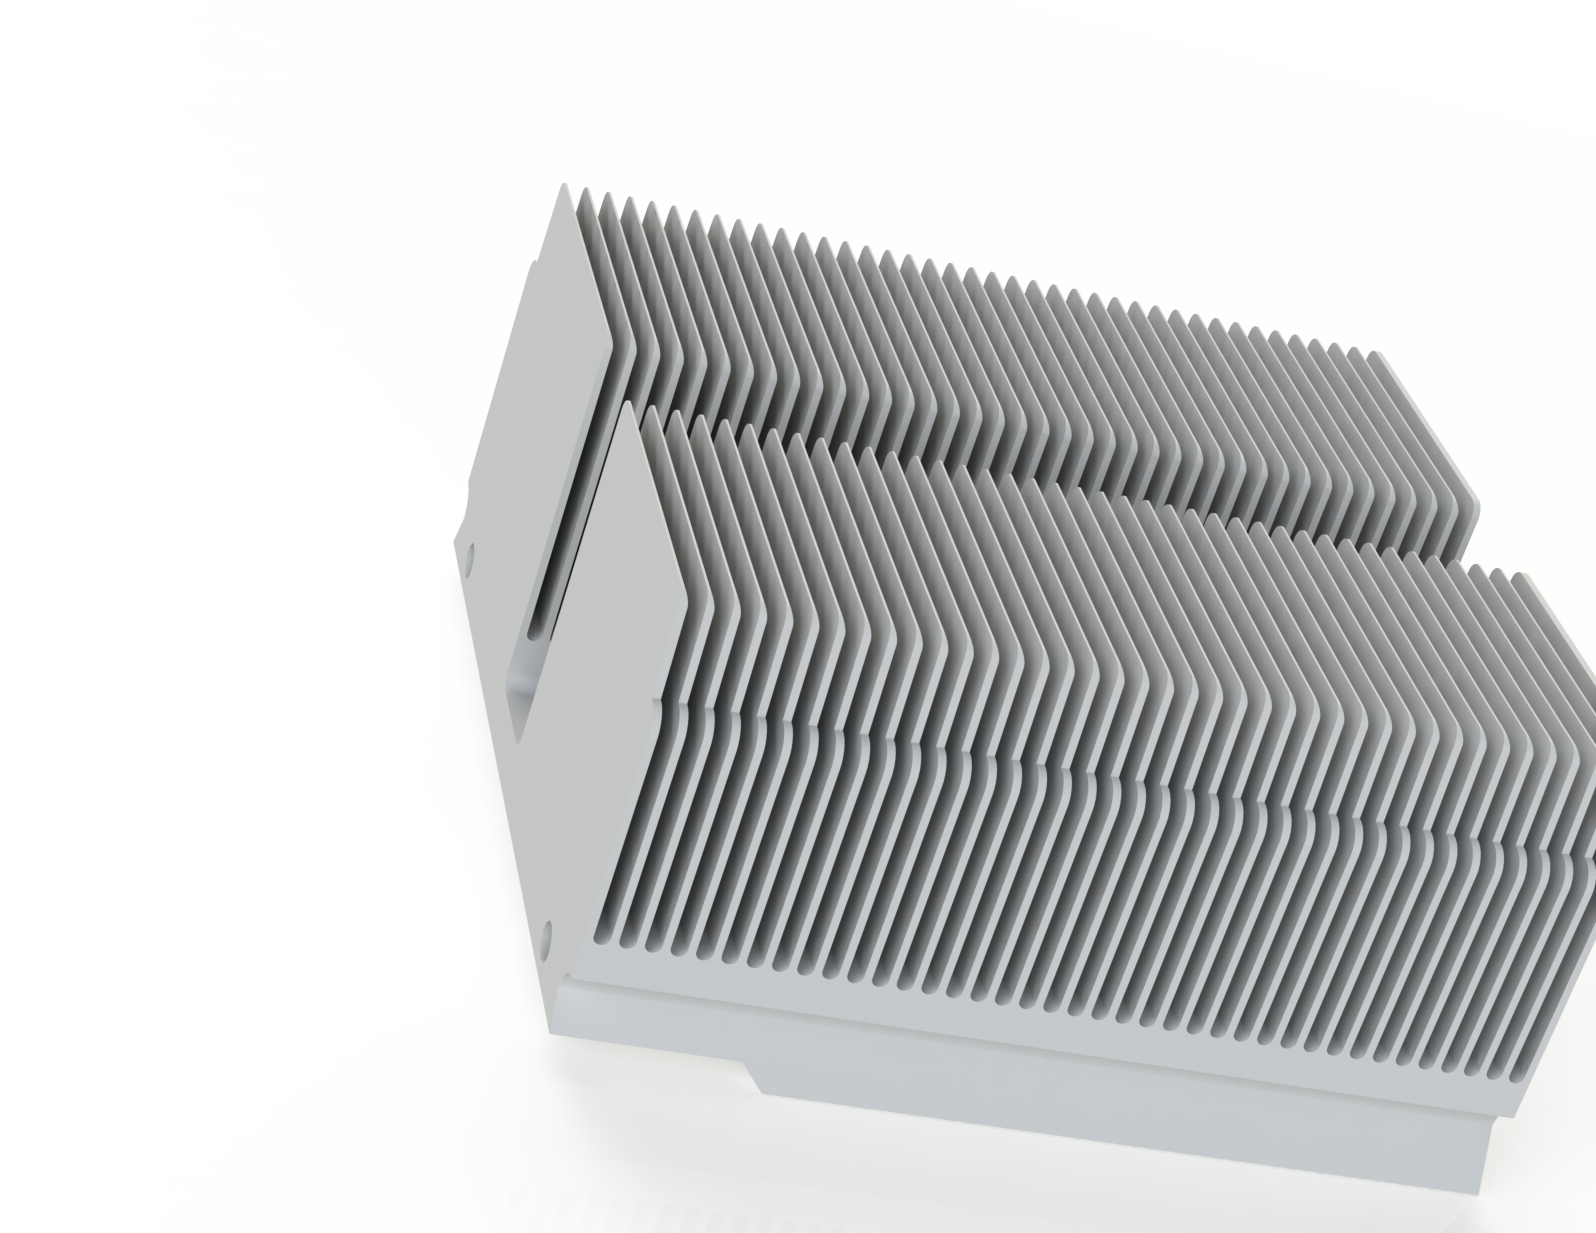
\includegraphics[width=0.7\linewidth]{C:/Users/Martin/Desktop/heatsink1}
			
			
		\end{figure}
		\vspace*{1cm}
		
			\vspace*{1cm}
		
		\textbf{Kølegitter}
		
		\textbf{Martin Knudsen}
		
		\vfill
		
		En undersøgelse af strømning, type og køleeffekt. 
		
		\vspace{2.0cm}
	\end{center}











\cleardoublepage												% Indsaetter tom side, saa naeste kapitel starter paa hoejre side (hvis noedvendigt)
%\include{formalia/titelblad}
\cleardoublepage
%\include{formalia/forord}
\cleardoublepage

%%%% Indholdsfortegnelse (TOC) %%%%

\phantomsection													% Kunstigt afsnit, som hyperlinks kan 'holde fast i'
\pdfbookmark[0]{Indholdsfortegnelse}{indhold}					% Tildeler en klikbar bookmark til den endelige PDF
\tableofcontents*												% Indholdsfortegnelsen (kaldet ToC) 

%\addtocontents{toc}{\protect\newpage}							% Fremtvinger sideskift i ToC hvis noedvendig (der hvor koden placeres)


\mainmatter														% Hovedindhold - nummereres fra side 1

%%%% Rapportindhold %%%% 										% Rapportindholdet boer IKKE indeholde broedtekst - KUN includede filer!

%% Indledende %%												% Opdel evt. i passende afsnit for overblikkets skyld

\section{Indledning}

Computere med dertilhørende køling og termodynamiske systemer fylder generelt meget i hverdagen for de fleste mennesker, men vi ved meget lidt om de termodynamiske processer i en PC.

Forfatterne interesserer sig for moderne højtydende PC-systemer, hvor køling i særdeleshed er en meget væsentlig faktor, herunder køling af den centrale regneenhed/processor (CPU - Central Processing Unit) samt evt. dedikerede grafik regneenhed/processorer (GPU - Graphics Processing Unit).

Det termodynamiske system vi har valgt at skrive om til dette projekt i termodynamik er processor-kølere som bruger tør atmosfærisk luft som kølemedie. Hvorfor det undersøges hvor meget hurtigere luft skal flyttes, for at give køling ved tvungen indvendig strømning en bedre køle evne end konvektion.

Vi har vi valgt at definere at systemgrænsen ligger mellem processoren og det køletekniske system, således at processoren og dens interface med det køletekniske system ligger udenfor det termodynamiske system vi beskriver. Således foregår der en strøm af energi ind over systemgrænsen og ud i den anden ende af system grænsen

Processoren kommer da til at definere energistrømmen ind i systemet og dermed den varme der skal transporteres ud af systemet for at det forbliver stationært ved maksimal belastning. 

Lauritzens og Eriksen, Termodynamik danner grundlaget for beregninger samt samt tabelopslag for diverse værdier i dette projekt.


\section[felt]
Der er 4 forskellige slags kølinger der vil blive undersøgt i denne rapport: 

\begin{itemize}
	\item kølegitre(Heatsink)
	\item Varmerør(heatpipes)
	\item blæser/fluid(el.andet flow)
	\item og fasekølinger
\end{itemize}


der er et overraskende stort udvalg af kølesystemer til processorer, og alt for mange til at de alle kan blive nævnt eller behandlet udtømmende i denne rapport. Men fælles for dem alle, er at de på en eller anden vis har fysisk forbindelse til processoren.
I denne rapport, vil vi undersøge og sammenligne effekten af de forskellige kølesystemer, når varmen afledes til sidsti kølesystemet. 
Vi vil ikke forholde os til køling og luftgennemstrømning af det kabinet som processor og kølesystem befinder sig i. Ikke fordi, der ikke sker termodynamiske ting i det, men fordi det umiddelbart, uden dybdegående inspektion, mere drejer sig om bortlednning af opvarmet luft end om bortleding af varme og måske ikke et direkte termodynamisk emne. 



%% Kontekst %%

\section[system/beskrivelse]

Fælles for alle PC kølesystemerne i denne rapport er den første komponent der leder varmen væk fra processoren.

Kølesystemet for en computerprocessor i første indsats består af en varmeledning af varme fra processor til kølesystem.
Ofte faciliteres varmetransmissionen ved hjælp af en pasta, for at maximere kontaktflade til kølesystemet og for at modvirke galvanisk tæring.
I kildelisten er to eksempler på en pasta, med konduktivitets værdier på 0,8 og 12,5 W/m*K.
imidlertid er intentionen med kølepasta, at optimere overflade kontakten imellem kølegitter og processor og ikke skabe et seperat lag, hvor der kan dannes ekstra varme modstand. Så laget af kølepasta vil her blive negligeret. På en moderne processor med millioner af transistorer, er det set at processoren kan smelte ved store belastninger. 

Så kort sagt, er det system vi undersøger et system der er afgrænset af interfacet til processoren og af bortledning af varme fra det sidste komponent af kølesystemet.
\section{Processor}

Den elektriske effekt P afsat i en CPU kan beskrives således :

 P = strømforbrug (I) * taktfrekvens (f) * kapacitans (C) .

 

I kølesystemet for en computerprocessor foregår den første varmetransmission som varmeledning fra processorens varmespreder til kølesystemet.

Ofte faciliteres denne varmetransmissionen af en kølepasta, som er med til at maksimere kontaktfladen til kølesystemet og som modvirker galvanisk tæring.

I kildelisten er inkluderet to eksempler på kølepasta, med konduktivitets værdier på hhv. 0,8 og 12,5 W/m*K.

Intentionen med kølepasta er at optimere kontakten mellem kølegitter og processor og undgå at der opstår små luftlommer, hvor der kan dannes ekstra varmemodstand. Dog vil laget af kølepasta her blive betragtet som liggende udenfor systemgrænsen.

De fleste kølegitre er lavet af aluminum, som har en varmekonduktivitet er på 229 W/m*K.

Vi antager et en dimensionel udbredelse af varme, stationært system med konstant varmestrøm. Vi antager ydermere konstant densitet og temperatur på den omgivende, tørre atmosfæriske luft.

Tykkelserne på godset i den retning varmen udbredes i er 0.5 mm for kølegitteret og regnes som en massiv væg, idet processoren regnes for at have en ens temperatur i hele sit areal.  Varmen forsimples til at udbredes i en retning og i et stationært system.  Med disse antagelser kan varmestrømmen igennem lamellerne beregnes.
Luften antages at flytte sig 0.01 m/s(c, hastighed)


%% Teknisk %%
\section{Gitter}

Fælles for alle 3 systemer er kølegitteret af aluminium, der er i kontakt med processoren. 
I simple systemer udgør kølegitteret den eneste part i kølesystemet som vi har defineret det og kan selvfølgelig bestå af andre materialer end aluminium. I nærværende rapport vil der dog tages udgangspunkt i aluminum.

Kølegitteret udnytter sit store overfladeareal til at bortlede varme ved konvektion fra et fast materiale (aluminium) til et fluid (tør atmosfærisk luft).
Således vil der være to termiske modstande, nemlig en varmeledningsmodstand i kølegitteret og en varmeovergangsmodstand fra fast stof til fluid.

En hyppig forekommende geometrisk struktur i et kølegitter er ribber eller lameller, der giver en naturlig strømning af den varme luft bort fra kølegitteret, hvor kun termodynamiske kræfter har indflyldelse på strømningen. Denne strømning foregår mellem to ribbe/lamel-vægge. 

Der præsenteres her en oversigt over de værdier der bruges i udregningerne: 

Der beregnes varmestrøm for konvektion og for stråling.

Dimensionerne for kølegitteret er importeret fra en partfil i Solidworks. %Kanalen for strømningen af luft der regnes for er d(1mm) bred og den hydraulisk diameter regnes som værende en snæver kanal, hvor L=2*a

$H = 20\ mm$, $b = 25,5\ mm$, $d = 1\ mm$, Areal $A_t = 93733.73\ mm^2$, $A_{lamel}= 500\ mm^2$  \\ 
Massen $m = 31,58 g$ \\
Varmekonduktiviten for aluminium, $\lambda_{al} = 229\ W/m*K$ \\  
Lameltykkelsen $\delta = 0.5\ mm.$  \\
Den specifikke varmekapacitet $c_{p} = 1.008\ kJ/kg*K$ \\
Strømningshastighed lodret, i lamellens længde på $c = 0.001\ m/s$ \\


Hvoraf varmekonduktiviteten $\alpha$ er fundet ved tabel opslag $\alpha = 21.8$ \\
Kinematisk viskositet er: $18.88$ og dynamisk viskositet = $16.92$  \\
Volumenudvidelseskoefficienten $\beta_luft = 3,2$ \\
 
Varmeledningsmodstanden : $R_l = \frac{\delta}{\lambda_{al}*A_{lamel}} = 4.281$ \\
Varmeovergangsmodstanden : $R_o = \frac{1}{\alpha_{tl}*A_{lamel}} = 89.394$ \\

Total termisk modstand er $R_{tot} = R_l + R_o = 92.225$ \\

\section{Beregninger}

For at udregne varmestrømmen $\phi$  bruges udtrykket \\ $\Phi = \alpha * A* (t\_{fl}-t\_v$ \\  også kendt som Newtons ligning. \\ 

Varmestrømmen $\phi$ udregnes ved ligningen Nu = $\frac{\alpha}*{\lambda}$ \\
Nu er Nusselts tal og findes herunder ved at udregne Reynolds(Re) og Prandtls(pr) tal.

Strømningsforholdende for luft(fluiden) imellem lamellerne i gitteret er fri indvendig strømning, idet lamellerne kan ses som kanalvægge og udgangen i en antaget lodret given retning er smal og bred med 3 åbne sider og derved tillader en fri udvikling af strømningen. Den hydrauliske diameter bruges og sættes lig med afstanden imellem 2 givne lameller. $\approx 0.5 mm$

Reference temperaturen udregnes til : 
\\$t_{film} = \frac{{t_{lamel}}+t_{fluid}}{2} => t_{film}=30$
\\Grasshofs tal Gr = $\frac{g*L^3*\beta*{\Delta\,t}}{\upsilon\,^2} = 8,771*10^4$
\\Prandtls tal Pl(opslag) => $Pr=0.69$

Der antages lodret laminar strømning af luften og Reynold tal undersøges for at få en idé om strømningsformen\\

$Re = \frac{c_{luft}*L_{hyd}}{\upsilon} = 2.648*10^{-5}$
%$ Ra = Gr*Pr = 6.052*10^4$ => \\ 

Den kritiske værdi for Re hvor strømningen overgår fra at være laminar til at blive turbulent er $10^9$.  Da ovenstående beregnede værdi af Re er meget mindre end den kritiske værdi, ses at der må være tale om laminar strømning over hele længden af en lamel, hvorfor strømningen ikke undersøges yderligere.

Hastighedsprofilen hvorved den opvarmede luft stiger til vejrs er udregnet til: 
$0.05*Re*L_{hd} = 0.001 $

Her følger et overblik over forksellene på to strømningsformer.

\subsection{Tvungen indvendig strømning}
Det medfører at Nusselts tal kan udregnes som \\ 
$Nu = 3,66+ \frac{0.0668*Re*Pr*\frac{D}{L_{lamel}}}{1+0.004*()\frac{D}{L_{lamel}}*k *Re*Pr})^{2/3} = 3.661$


%Den kritisk værdi findes da ved: $Nu_m = C*Ra^4$

og $ \Phi_{tis} = \alpha*A(t_{fl}-t_v =>2.597*10^6 W $\\ 
justeret til milimeter ved udtrykket: $\frac{\Phi = \alpha*A*(t_{fl}-t_v}{10^6} =>160,4 W$

Hvor luftens hastigheds profil er fuldt udviklet efter :
$0,05*Re = 0,03 mm$

samtlige lammeler afgiver da $0,75 w* 40 \approx 30 W$ i varmestrøm til luften der passerer. 

\subsection{Fri Konvektion}

Fri konvektion er et lidt tænkt scenerie er lidt begrænset i sin relevans, men dog brugbar for enkelt lameller og dele af kølegitteret.
$Nu_{fri} = (\frac{Gr_{L}}{4})^4 * (\frac{0,75*Pr^1/2}{(0.609+1,221*Pr^1/2+1,238*Pr)})^1/4$
og ledetallet $\alpha_{fri} = 2,768*10^3$

Varmestrømmen $\phi_{fri}=169,37$  







%% Afrunding %%

%\section{Konklusion}

Et varmegitter af aluminium forekommer umiddelbart at være en relativt effektiv måde at aflede varmen på. 
Den store hindring i varmetransmissionenforekommer at være overgangsmodstanden for luft. 
Materialet lader ikke til at gøre en synderlig forskel, dog skal det bemærkes at aluminium er et af de mest varmeledende materialer, billigt, let og nemt at forarbejde.

Ulempen ved sådan en konstruktion her er, at fluidets filmlag er relativt tykt og har laminart flow, hvorfor luftudskiftningen er lidt langsom og mindre effektiv i konvektion. 
Men materialet er generelt underordnet ift. laminart/turbulent flow og det samlede overfladeareal, hvorfor det giver god mening at aluminium bruges i vid udstrækning til pc kølesystemer. 

Hvis angelsen om at opdrifthastigheden på luft er $0,5mm$
Skal luften flyttes ca. 8 gange hurtigere ved at bruge en blæser, inden filmlaget bliver brudt tilstrækkeligt til at øge varmestrømmen $\phi$.


%%%% Kilder %%%%

\begingroup
	\raggedright
	\bibliography{bibtex/litteratur}							% Litteraturlisten inkluderes
\endgroup


%%%% Fixme-listen %%%%

\newpage														% Ny side til Fixme-listen
\listoffixmes													% Fixme-listen - fjernes til sidst i projektet med "%"


%%%% Appendiks %%%%

\appendix														% Appendiks/bilag start - giver chapter bogstaver i stedet for tal
\clearforchapter												% Sikrer at pagestylen aktiveres paa den rigtige side
\phantomsection													% Kunstigt afsnit, som hyperlinks kan 'holde fast i'
\pdfbookmark[0]{Appendiks}{appendiks}							% Tildeler en klikbar bookmark til den endelige PDF

%% Indstillinger for appendiks (deaktiveret med "%") %%

%\pagestyle{empty}												% Sidehoved/-fod for standardsider aendres til tom for appendiks
%\aliaspagestyle{chapter}{empty}								% Sidehoved/-fod for kapitelsider aendres til tom for appendiks
%\settocdepth{chapter}											% Kun kapitel-niveau vises i ToC
%\addtocontents{toc}{\protect\cftpagenumbersoff{chapter}}		% Sidetal for kapitler fjernes i ToC

%% Filer til appendiks %%

%\include{appendiks/appendiks1}


%%%% Bilag %%%%

%\phantomsection												% Kunstigt afsnit, som hyperlinks kan 'holde fast i'
%\addcontentsline{toc}{chapter}{Bilag A \ Navn} 				% Manuelle indgange i indholdsfortegnelsen (naar \includepdf bruges)

%\includepdf[pages={x-y}]{filnavn}								% Inkluder eksterne bilag med \includepdf[pages={x-y}]{filnavn}


\end{document}													% Slutter dokumentet - obligatorisk


